\documentclass[11pt,a4paper]{article}
\usepackage[margin=2cm]{geometry}

%% adding graphics
\usepackage{graphicx}
%% nicer tables
\usepackage{booktabs}
%% rotate pages for landscape
\usepackage{pdflscape}
%% nice grid layouts for latex figures
\usepackage{subcaption}

\begin{document}

\title{Automatic Flow-based Classification of B-Cell Lymphoma}


\section{Introduction}

Flowcytometry aids in the detection and classification of lymphatic disorders, but current multi-channel flow data is hampered by the limitations of human interpretability.
Statistical preprocessing promises to enable the description of higher-dimensional relationships in measured events.
Extending previous work on preprocessing and classification of flowcytometry data, we created a proof-of-concept approach for unattended debris-removal and classification on a large dataset of B-Cell-Lymphoma.

\section{Aims}

Design and implementation of an automated analysis process for determination of B-Cell-Lymphoma diagnoses from flowcytometry data of peripheral blood and bone-marrow samples.


\section{Methods}

For the initial analysis flow cytometry data was obtained from routine flow panels for B-Cell-Lymphoma from the years 2016--2018. A total of xxx patients have been obtained. The given cohort contained 9 different B-Cell lymphoma subtypes, as well as non-pathological normal cases.

FCS data is prepared with removal of some zero values and limitation of data to shared markers. A CD45 positive, side scatter negative cell population is automatically selected in each case using a DBSCAN-based (density based spatial clustering of applications with noise) population search on an individually generated SOM (self-organizing map), representing the data.

From each disease entity a small subset of cases is selected for the generation of the consensus SOM, which is trained on small subsets of all included diagnoses. The fitted model is used to transform invididual cases into their distribution on the SOM.

The distribution information serves as input to the classification process for the prediction of individual labels. For which currently a sequential neural network and a random decision tree have been implemented.

\section{Results}

Initial 9-class classifications obtained accuracies of XX\% across 5 generated maps, with classification calculated in 10-fold cross-validation. Cohorts were at maximum limited to XX samples, while smaller cohorts were left at their respective sizes.
Hierarchical clustering showed similarities between CLL/PL and mantle cell lymphoma, as well as between lymphoplasmocytic lymphoma and marginal cell lymphoma.


\begin{figure}
   \centering
   \raisebox{-0.5\height}{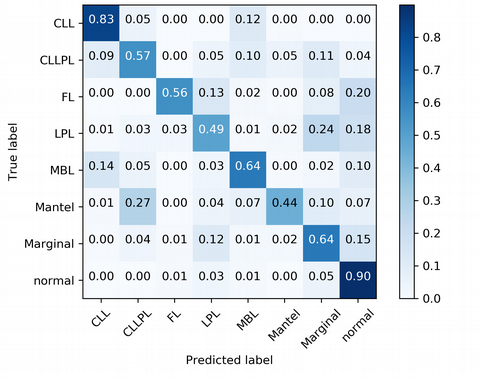
\includegraphics[width=0.5\textwidth]{dendro_confusion}}
   \raisebox{-0.5\height}{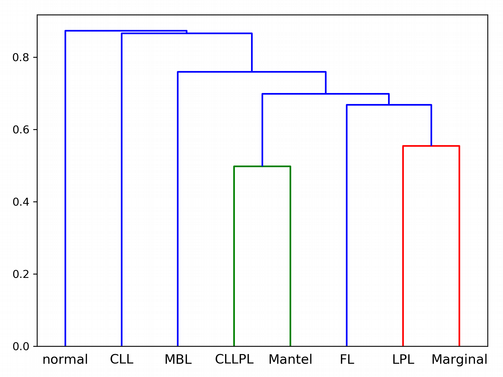
\includegraphics[width=0.4\textwidth]{dendro}}
   \caption{Hierarchical clustering on confusion matrix values. Groupings are created per column, with similar columns grouped closer.}
\end{figure}


%% tsne results and som for normal vs cll
%% pregating w/ dbscan
%% neural net classification normal cll
%% results for xxx different lymphoma entities
%% clustering joint entities, similarity in classification

\begin{figure}
   \centering
   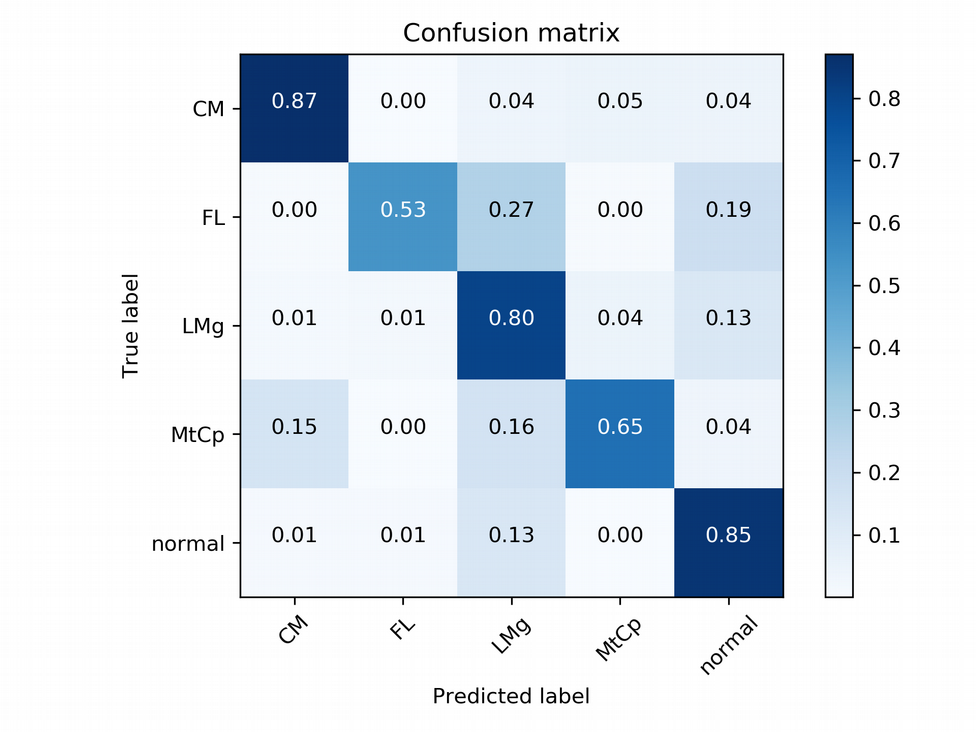
\includegraphics[width=0.6\textwidth]{classification}
   \caption{Classification results for merged groups.}
\end{figure}

\begin{figure}
   \centering
   \raisebox{-0.5\height}{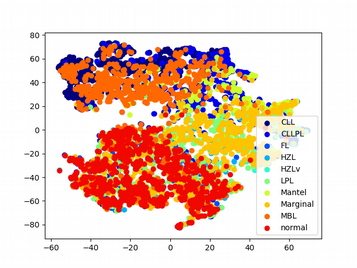
\includegraphics[width=0.45\textwidth]{tsne_t1}}
   \raisebox{-0.5\height}{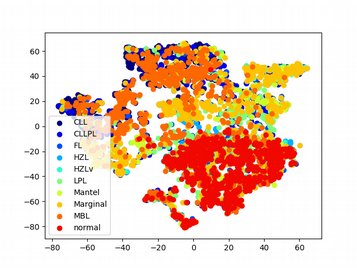
\includegraphics[width=0.45\textwidth]{tsne_t2}}
   \caption{tSNE visualization of upsampling histogram data from separated maps for tube 1 and tube 2.}
\end{figure}

\begin{figure}
   \centering
   \raisebox{-0.5\height}{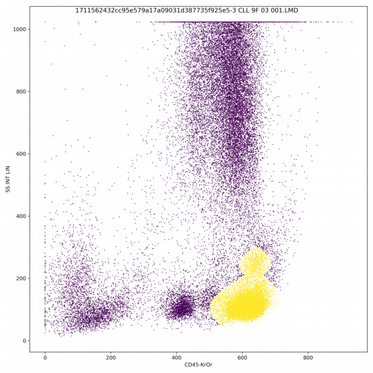
\includegraphics[width=0.45\textwidth]{pregating_1}}
   \raisebox{-0.5\height}{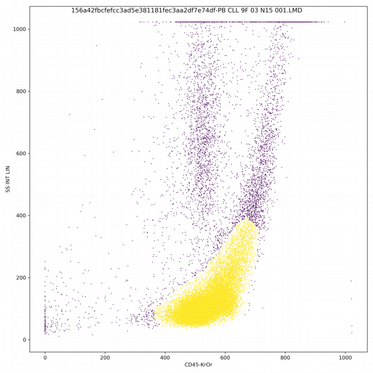
\includegraphics[width=0.45\textwidth]{pregating_2}}
   \caption{Visualization of pregating process for CD45 positive, side scatter negative cell populations. The yellow cell population will be selected for further processing, all other events will be discarded.}
\end{figure}

\section{Conclusions}

Our classification prototype shows the viability for automated classification on large routine diagnostics dataset.
Further improvements to flexibility and generalizability of the approach can be made to encompass incomplete and changing panels, as well as testing of a more diverse patient set, including cases with diagnoses outside the diagnostic target of given panel, such as patients later diagnosed with myeloic leukemias.

%% viability of automated conclusions

%% required further development

%% sources for error

%% combination approaches

%% challenges regarding changing data qualities etc

\end{document}
